\documentclass[12pt]{article}
\usepackage[english]{babel}
\usepackage{subcaption}
\usepackage{hyperref}
\usepackage{graphicx}
\graphicspath{{images/}}
\usepackage{geometry}
 \geometry{
 a4paper,
 total={170mm,257mm},
 left=20mm,
 top=20mm,
 }
\begin{document}

\section{Problem1}
In the first problem, we are supposed to enhance the quality of the given input video.

\subsection{Method Employed}
\begin{enumerate}
\item First we converted the image into gray and analyzed the pixel distribution using histogram and got the following output.

\begin{figure}[h]
    \centering
    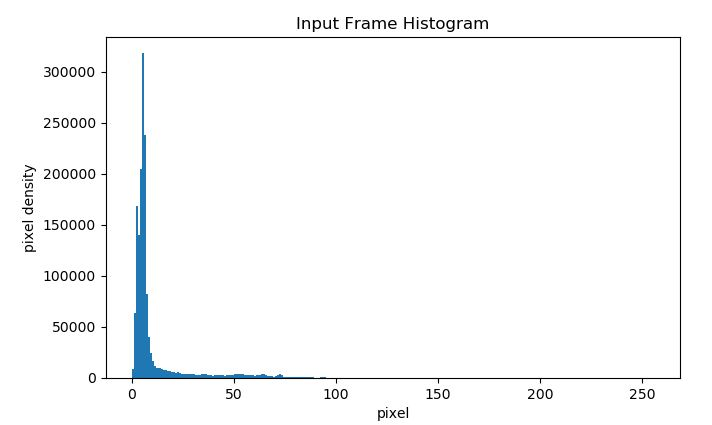
\includegraphics[width=12cm]{inputhistogramoutput}
    \caption{Input frame Histogram output}
    \label{fig:inputhistogramoutput}
\end{figure}

We saw high density of pixels within the range 0-50. The goal was to increase the contrast by distributing the pixel density evenly between 0-255.

\item Initially we tried to improve the quality of the video using histogram equalization. The output certainly increased the brightness of the video but at the same time amplified also noise.

\begin{figure}[h]
    \centering
    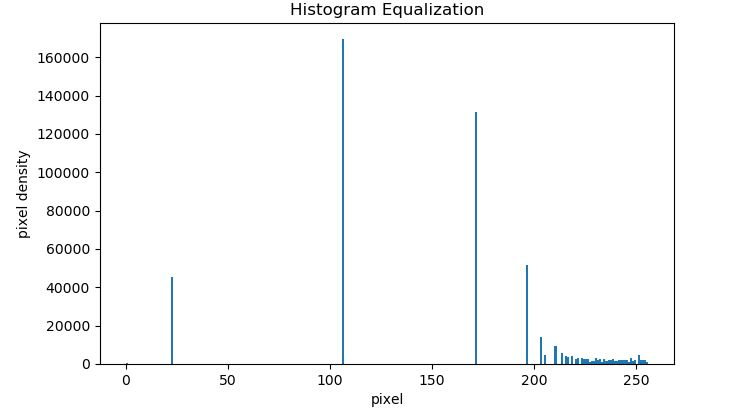
\includegraphics[width=12cm]{histogramequalization}
    \caption{Histogram Equalization output}
    \label{fig:histogramequalization}
\end{figure}

After performing histogram equalization, the pixel density was distributed but resulted in noise amplification clearly seen between pixel range 100-150. We tried to decrease the noise by using filters but could not decrease the noise.

\item We employed gamma correction. This method could increase the quality by could not increase the contrast.
\begin{figure}[h]
    \centering
    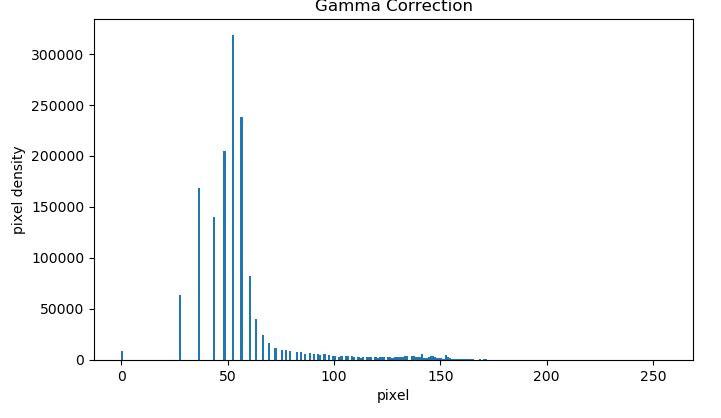
\includegraphics[width=12cm]{gammahist}
    \caption{Gamma Correction output}
    \label{fig:gammahist}
\end{figure}

\item Then we multiplied each pixel with $\alpha$ and added by $\beta$. We found this method increased the contrast while decreasing the noise compared to histogram equalization. The histogram output of this method is given below:

\begin{figure}[h]
    \centering
    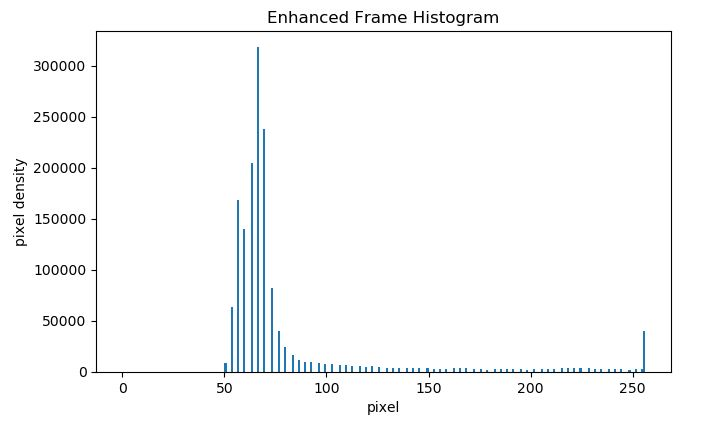
\includegraphics[width=12cm]{enhancedhistogram}
    \caption{Enhanced Frame output}
    \label{fig:enhancedhistogram}
\end{figure}
We can see that the pixel density is distributed and at 255 there is sharp rise in the pixel density which is indicative of increase in contrast of the image. The equation below clearly outlines this method:
\begin{equation}
	NewFrame = \alpha*OldImage + \beta
\end{equation}
\end{enumerate}

\subsection{Outputs Obtained}
\begin{enumerate}
\item The outputs are snippets of one of the input frame taken from the video. The input frame considered: 
\begin{figure}[h]
    \centering
    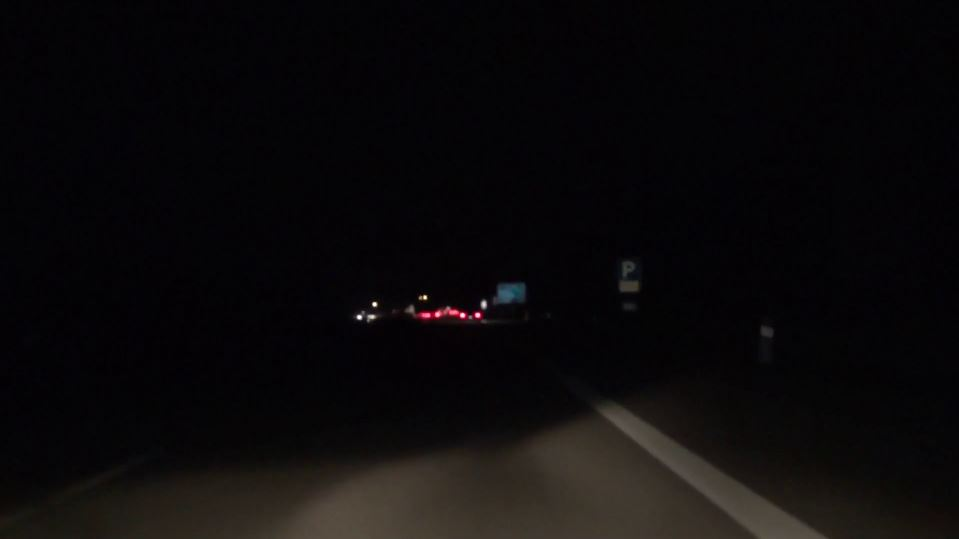
\includegraphics[width=14cm]{inputframe}
    \caption{Input Frame}
    \label{fig:inputframe}
\end{figure}

\item Histogram Equalization Output: This contains the snippet output obtained by employing histogram equalization. We can see that the contrast is improved at the same time noise is also improved.
\begin{figure}[h]
    \centering
    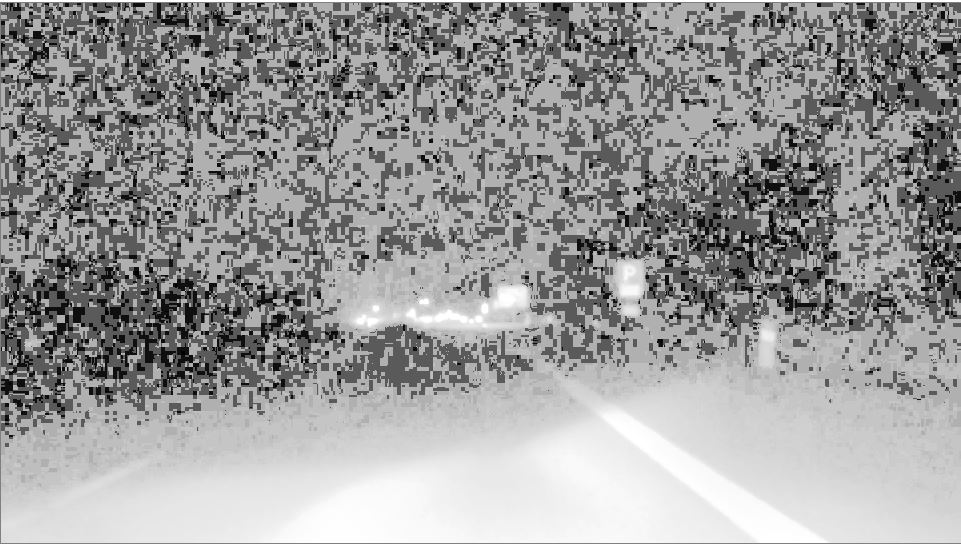
\includegraphics[width=14cm]{histequvideo}
    \caption{Histogram Equalization output}
    \label{fig:histequvideo}
\end{figure}

\newpage
\item Gamma Correction Output: This contains the snippet output obtained by employing Gamma correction. We can see that contrast is not improved.

\begin{figure}[h]
    \centering
    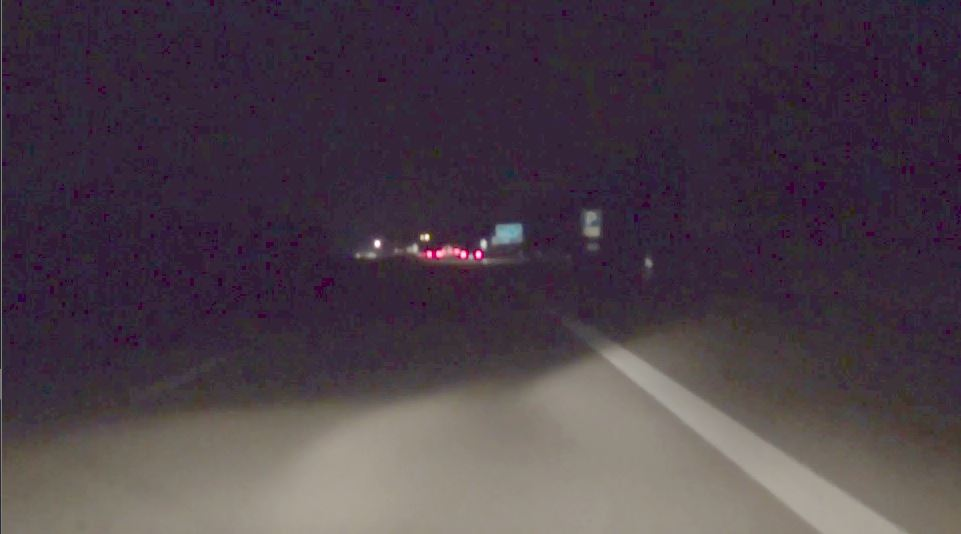
\includegraphics[width=14cm]{gammavideo}
    \caption{Gamma Correction output}
    \label{fig:gammavideo}
\end{figure}

\item Method Employed Output: This is the snippet of the image frame from the enhanced video. We improved the contrast and decreased the noise levels.We can clearly see the lanes and road signs from the enhanced frame.
\begin{figure}[h]
    \centering
    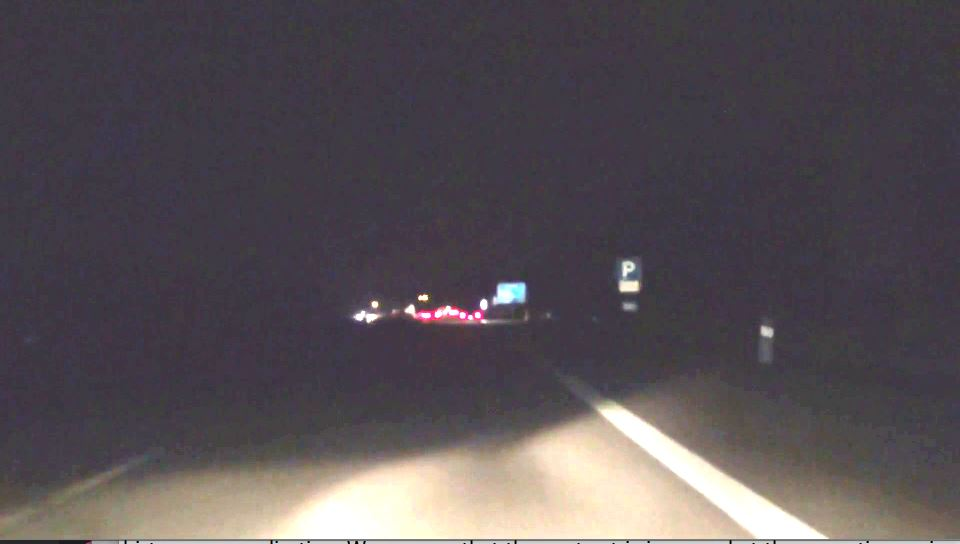
\includegraphics[width=14cm]{enhancedvideosnippet}
    \caption{Enhanced frame output}
    \label{fig:enhancedvideosnippet}
\end{figure}
\end{enumerate}

\subsection{Accessing output video} 
For accessing the full length output video please click on this \href{https://drive.google.com/drive/folders/1f6jBcJo96DZhwxBkdezf6MwAXwktGqS-?usp=sharing}{\underline{link}}.

\subsection{References:}
\begin{enumerate}
\item \href{https://docs.opencv.org/3.4/d3/dc1/tutorial_basic_linear_transform.html}{\underline{Opencv documentation for improving the contrast and quality of the image.}}
\end{enumerate}

\section{Problem 2}
In this problem, we are given one video and list of images and we need to provide two videos detecting lanes,

\subsection{Procedure employed}
\subsubsection{Step1: Prepare the Input}
\begin{enumerate}
\item For given list of images we had an additional step of first converting them into a video

\item First we used in-build Opencv function to undistort the image using the given camera parameters.

\item Then we used Gaussian filter to reduce noise in the image.

\item Then we used in-build Opencv canny edge detection function to extract the edges from the image.

\item For region of interest, we cropped the upper part of the image which is the sky and made lower part of the image as  our region of interest(ROI).
\end{enumerate}
\subsubsection{Step2: Detect Lane Candidates - Histogram of Lane Pixels}
\begin{enumerate}
\item First we took 4 points, 2  from each lines to compute the homography.

\item Then using in-built Opencv $warpperspective()$ function, we warped the image and got the top view of the road.

\item We are only interested in lanes. So we removed unwanted color pixels by converting RGB image to HSL image. This will highlight only the lanes.

\item There were two colors with high pixel density on the HSL image which were white and yellow. We used the concept of masking to separate these two colors. By using $inrange()$ function to separate the yellow and white pixels in mask1 and mask2 separately.

Mask1 contains only the white pixels of the lane.
Mask2 contains only the yellow pixels of the lane.

\item Mask1 and Mask2 are now separate anded with the image with edges(Output of Canny) using $bitwiseand()$ function in opencv. The resulting two images will contain only lanes which are again ored using $bitwiseor()$ function to get a single color image consisting of only lanes with edges. 

\item Now we need to know the indexes of the pixel which corresponds to white and yellow pixels. For this, we converted the HSL image to gray image and obtained histogram of the image.

\item On histogram we see two peaks, which correspond to white and yellow pixels got from the lower half the image. We divided the lower half of the lower half of the image into two smaller frames. These smaller frames are divided into two categories based on their position with respect to the midpoint of the histogram. The frames on the left of the midpoint are for left (yellow) lane and right are for right (white) lane. The height of these frames depends on how much we are dividing the lower half of the image.

\item We create two lists for yellow and white lanes. We loop through these smaller frames and if any pixel is found with non-zero value we add the indexes into the corresponding yellow and white list.

\item We do this for the entire lower half of all the frames of the video.

\item Then we use $ployfit()$ function to fit a polynomial along the white and yellow lines. Then $fillpoly()$ function fills the polynomial between the white and yellow lanes.

\section{Homography}

\item In our code we have made used of homography in which we have manualy obtained the 4 points in order to do the homography transfromation. In this method we have manually obtained minimum of 4 points required for the homography transformation.   


\end{enumerate}
\end{document}

